\section{Architecture}

\begin{figure}[t]
   \begin{center}
     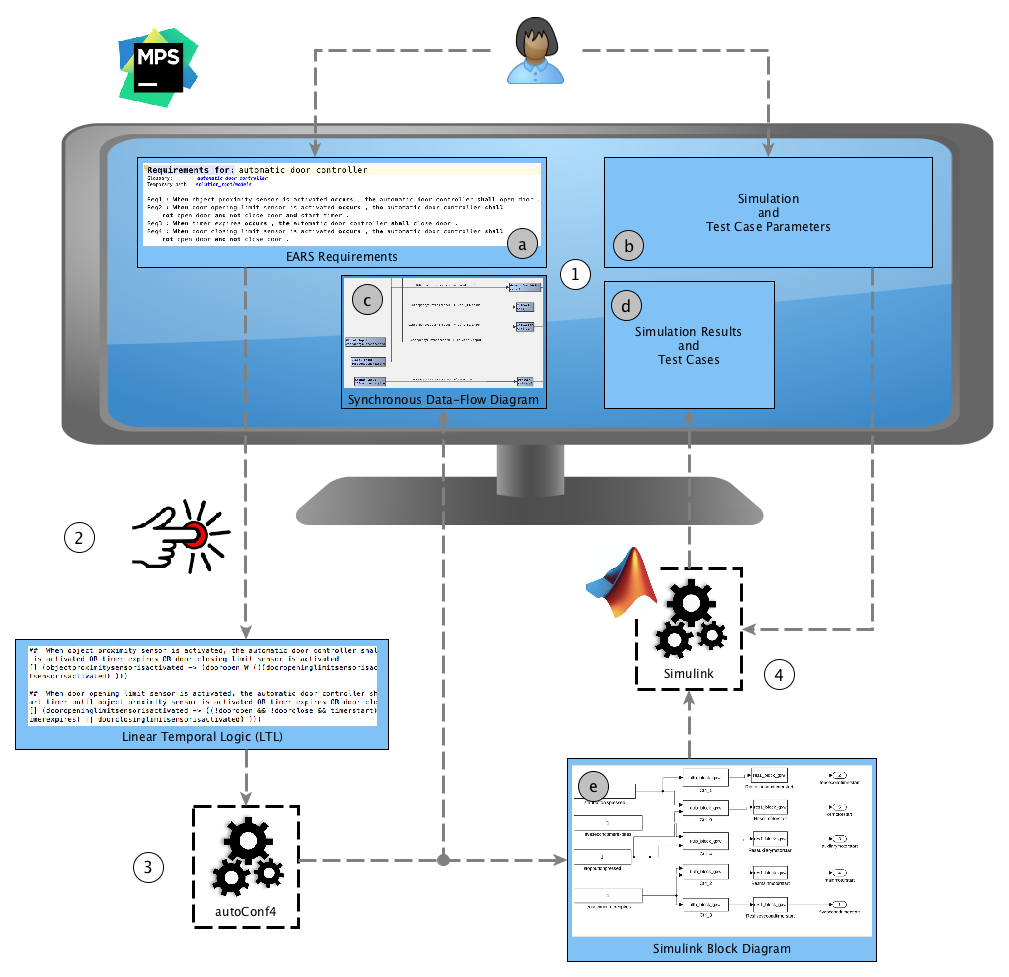
\includegraphics[width=1\textwidth]{images/toolchain.png}
     \caption{The \textsf{EARS-CTRL} Tool Chain}
     \label{fig:ears_ctrl_toolchain}
   \end{center}
 \end{figure}
 
In figure~\ref{fig:ears_ctrl_toolchain} we depict the architecture of the
\textsf{EARS-CTRL} tool. In the following paragraphs we will provide to the
reader a brief description of the main components of the tool's architecture,
how those components have been implemented and which artifacts those
components interchange. 
 
\paragraph{1. Requirements and Glossary Editor\\\\} 

Both the requirements and the glossary editors have been built as
domain-specific languages in the MPS meta-editing tool. The languages are mostly
composed of an abstract syntax (also known as meta-model) and a concrete syntax
which allows displaying and editing the information in a neat fashion, as
depicted in figures~\ref{fig:ears_reqs} and ~\ref{fig:ears_glossary}. In order
to build a new set of requirements or a glossary the requirements engineer
simply builds an instance (also known as a model) of the corresponding language.
Note that because MPS is a projectional editor the abstract syntax is directly
edited in the model. A direct consequence of this is for example the fact that
when a glossary component's name is updated in the glossary editor, that term
will be immediately updated in any requirements that refer to that component
name. This is because requirements directly refer to the component names defined
in the glossary.

\paragraph{2. From EARS to Lineal Temporal Logic\\\\}

\textsf{EARS-CTRL} requirements can be translated mostly in a straightforward
fashion from the English language into LTL. Take for instance requirement
``Req1'' from figure~\ref{fig:ears_reqs}:

\begin{center}
\textbf{When} \emph{object proximity sensor is activated} \textbf{then the} \emph{automatic door controller} \textbf{shall}
\emph{open door}.
\end{center}

 This requirement translates into the following LTL formula:
 
 $$[] (objectproximitysensorisactivated \rightarrow dooropen)$$
 
 which, if one takes into consideration the semantics of the $\rightarrow$
 operator as ``implies'', is the expected logical meaning of ``Req1''. However,
 if one translates the whole set of requirements for the automatic door in
 \ref{fig:ears_reqs} into LTL, the result for ``Req1" will be as follows:

\begin{align*}
[] (objectproximity&sensorisactivated \rightarrow\\
 &(dooropen\,W\,(((dooropeninglimitsensorisactivated \lor timerexpires\\
 & \lor doorclosinglimitsensorisactivated )))
\end{align*}
 

\paragraph{3. Synthesizing a Controller using \textsf{autoConf4}\\\\}

\paragraph{4. Simulation and Test Case Generation Control Panel\\\\}

Say here how the exploration mechanism works by simulating steps iteratively to
build the test cases according to the test set parameterization.

\paragraph{5. Simulation and Test Generation using Simulink\\\\}

Talk about how blocks from Simulink are composed together to allow building the
expected behavior. Some blocks had to be purposefully build to allow simulation
to happen. This is done via a script that loads the model into Simulink \ldots
